\documentclass[a4paper,12pt]{ctexart}

\usepackage[left=2.3cm,right=2.3cm,top=2.7cm,bottom=2.7cm]{geometry}
\usepackage{graphicx}
\usepackage{xcolor}
\usepackage{float}
\usepackage{booktabs}
\usepackage{array}
\usepackage{amsmath,amssymb,bm}
\usepackage{fancyhdr}
\usepackage{lastpage}
\usepackage{hyperref}
\usepackage{pgfplots}
\usepackage{listings}
\usepackage{algorithm}
\usepackage{algorithmicx}
\usepackage{algpseudocode}

\pgfplotsset{compat=1.18}

\hypersetup{
    colorlinks=true,
    linkcolor=black,
    urlcolor=blue,
    citecolor=black
}

\lstset{
    language=C++,
    breaklines=true,
    basicstyle=\small\ttfamily,
    keywordstyle=\color{blue!70}\bfseries,
    commentstyle=\color{green!40!black},
    stringstyle=\color{red!60!black},
    numbers=left,
    numberstyle=\tiny\color{blue!50},
    frame=single,
    columns=flexible,
    showstringspaces=false
}

\floatname{algorithm}{Algorithm}
\renewcommand{\algorithmicrequire}{\textbf{Input:}}
\renewcommand{\algorithmicensure}{\textbf{Output:}}
\renewcommand{\contentsname}{目录}
\renewcommand{\figurename}{图}
\renewcommand{\tablename}{表}

\pagestyle{fancy}
\fancyhf{}
\lhead{\kaishu \leftmark}
\rhead{\kaishu 并行程序设计实验报告}
\cfoot{\thepage\ / \pageref{LastPage}}
\renewcommand{\headrulewidth}{0.1pt}
\renewcommand{\footrulewidth}{0pt}
\setcounter{tocdepth}{2}

\begin{document}

\begin{titlepage}
    \begin{center}
        
\includegraphics[width=0.8\textwidth]{assets/NKU.png}\\[1cm]

        \vspace{20mm}

        {\huge\bfseries\kaishu 计算机学院\par}
        \vspace{0.5cm}
        {\huge\bfseries\kaishu 并行程序设计实验报告\par}
        \vspace{2.3cm}
        {\Huge\bfseries\kaishu 多线程 NTT 实验\par}

        \vspace{\fill}

        {\LARGE\kaishu 姓名：马禹翔\par}
        \vspace{0.5cm}
        {\LARGE\kaishu 学号：2410933\par}
        \vspace{0.5cm}
        {\LARGE\kaishu 专业：计算机科学与技术\par}

        \vfill
        {\Large \today\par}
    \end{center}
\end{titlepage}

\tableofcontents
\thispagestyle{plain}
\clearpage

\section{实验目的}

本次实验选择 NTT 作为 pthread 和 OpenMP 多线程编程的研究对象。实验沿用了 Lab2 中的串行 NTT 基线、模数选择和测试规模，主要完成 pthread 和 OpenMP 两种多线程实现，并比较不同问题规模、不同线程数下的性能变化。

实验目标如下：
\begin{enumerate}
  \item 理解 NTT 蝶形运算中的数据依赖关系，找出哪些计算单元可以放心地交给不同线程；
  \item 实现串行 NTT、pthread NTT 和 OpenMP NTT，并保证三者的卷积结果完全一致；
  \item 自己设计 pthread 线程同步方案，避免每一层变换中出现数据竞争；
  \item 测试不同多项式规模和线程数下的运行时间、加速比和正确性；
  \item 结合实验数据分析线程创建、同步、负载划分和 OpenMP 调度对性能的影响。
\end{enumerate}

\section{实验原理}

\subsection{NTT 卷积}

给定两个长度为 $n$ 的多项式
\[
A(x)=\sum_{i=0}^{n-1}a_i x^i,\quad B(x)=\sum_{i=0}^{n-1}b_i x^i
\]
直接卷积复杂度为 $O(n^2)$。NTT 将多项式从系数表示转换到模数域下的点值表示，在点值域逐点相乘后再通过逆变换恢复系数，复杂度降为 $O(n\log n)$。

本实验使用的模数和原根为
\[
p=7340033=7\times 2^{20}+1,\quad g=3
\]
这个模数可以支持本实验规模下的二次幂长度 NTT，而且也是 Lab2 中采用的 NTT 友好模数，因此两次实验的输入设置和正确性基准可以保持一致。

\subsection{蝶形运算与并行性}

迭代式 NTT 的核心循环如下：

\begin{lstlisting}[title=串行 NTT 核心循环]
for (int len = 2; len <= n; len <<= 1) {
    int half = len >> 1;
    int wlen = qpow(g, (p - 1) / len);
    for (int base = 0; base < n; base += len) {
        int w = 1;
        for (int k = 0; k < half; k++) {
            int u = a[base + k];
            int v = a[base + k + half] * w % p;
            a[base + k] = (u + v) % p;
            a[base + k + half] = (u - v + p) % p;
            w = w * wlen % p;
        }
    }
}
\end{lstlisting}

分析 NTT 循环可以发现，同一层中每个蝶形运算只读写 $a[base+k]$ 和 $a[base+k+half]$ 两个位置。对于固定的 $len$，不同蝶形运算覆盖的数组位置互不重叠，因此同一层内的所有蝶形运算可以并行执行。但层与层之间存在依赖，当前层没有全部完成时，下一层不能提前开始。

基于这一点，将同一层的 $n/2$ 个蝶形运算线性编号：
\[
task = block \times half + k
\]
其中
\[
block=\left\lfloor task/half\right\rfloor,\quad k=task\bmod half
\]
然后把 task 按静态轮转方式分配给各个线程。这样做比较直接，也方便保证每个线程拿到的任务数量尽量接近。

\section{并行算法设计}

\subsection{pthread 采用的优化方式}

本实验 pthread 部分采用的是朴素多线程优化。具体来说，没有改变 NTT 的二分蝶形结构，也没有做四分 NTT 或多模数 CRT 合并，而是直接利用同一层 butterfly 之间互不依赖的特点，将同一层的蝶形运算划分给多个线程执行。这种方法实现复杂度相对较低，也最适合与 OpenMP 版本做一一对应的性能比较。

实验文档中 NTT 选题的进阶要求主要包括多分多线程优化和 CRT 多线程优化。多分优化可以理解为把连续两层二分蝶形合并成一次四路归并，从而减少层数和同步次数；但它需要重新处理四点 butterfly 的旋转因子，并且在长度不是 $4^k$ 时要额外预处理第一层或最后一层。为了保证主实验代码的正确性和与 Lab2 串行基线的可比性，本实验没有把四分 NTT 放入主测试表，而是在进阶尝试中分析其可行性。CRT 多线程优化主要面向大模数 NTT，而当前课程框架中模数参数仍以 \texttt{int} 读入，第四组大模数已经超过整型范围，所以这部分没有作为本次实现重点。

\subsection{pthread 实现}

pthread 版本采用的是静态线程的思想：每次 NTT 变换创建固定数量的工作线程，线程函数内部完成所有层的蝶形运算。每一层设置两个同步点：
\begin{enumerate}
  \item 0 号线程生成当前层旋转因子表后，所有线程等待；
  \item 所有线程完成当前层 butterfly 后，再同步进入下一层。
\end{enumerate}

一开始我考虑直接使用 \texttt{pthread\_barrier\_t}，但 Windows 下不同 pthread 环境对它的支持不完全一致。为了让代码更稳妥，我最后用 \texttt{pthread\_mutex\_t} 和 \texttt{pthread\_cond\_t} 自己实现了一个可复用 barrier。

\begin{lstlisting}[title=pthread 工作线程核心]
for (int len = 2; len <= n; len <<= 1) {
    int half = len >> 1;
    if (tid == 0) {
        int wlen = mod_pow(G, (MOD - 1) / len);
        if (invert) wlen = mod_pow(wlen, MOD - 2);
        roots[0] = 1;
        for (int i = 1; i < half; i++)
            roots[i] = mul_mod(roots[i - 1], wlen);
    }
    barrier.wait();

    for (int task = tid; task < n / 2; task += thread_count) {
        int block = task / half;
        int k = task - block * half;
        int base = block * len;
        // butterfly
    }
    barrier.wait();
}
\end{lstlisting}

这种划分方式的优点是负载比较均衡，每个线程处理的 task 数量最多只相差 1。由于每个 task 写入的位置唯一，计算主体不需要加互斥锁；只在层边界进行同步，也可以把同步开销控制在相对少的位置。

\subsection{OpenMP 实现}

OpenMP 实验文档中强调，可以在外层创建并行区域，避免在循环中反复创建和销毁线程。因此 OpenMP 版本没有在每一层单独写 \texttt{parallel for}，而是使用一个外层 \texttt{parallel} 区域包住整个 NTT 主循环；每一层中用 \texttt{single} 生成旋转因子表，再用 \texttt{for schedule(static)} 并行化同一层的 task 循环。

OpenMP 版本和 pthread 版本采用相同的 task 编号方式，所以二者在算法层面是一致的，主要差异来自线程管理方式、同步方式和运行时调度开销。

\begin{lstlisting}[title=OpenMP 核心循环]
#pragma omp parallel num_threads(thread_count)
{
    for (int len = 2; len <= n; len <<= 1) {
        #pragma omp single
        {
            // generate
        }

        #pragma omp for schedule(static)
        for (int task = 0; task < n / 2; task++) {
            // butterfly
        }
    }
}
\end{lstlisting}

\section{实验环境}

实验平台如下：

\begin{table}[H]
\centering
\begin{tabular}{ll}
\toprule
项目 & 配置 \\
\midrule
操作系统 & Windows \\
编译器 & MSYS2 UCRT64 g++ 15.2.0 \\
语言标准 & C++17 \\
编译选项 & \texttt{-O2 -std=c++17 -fopenmp -pthread} \\
测试线程数 & 1, 2, 4, 8 \\
测试规模 & 1024, 4096, 16384, 65536, 262144 \\
\bottomrule
\end{tabular}
\caption{实验环境与参数}
\end{table}

编译和运行命令如下：
\begin{lstlisting}[language=bash]
g++ -O2 -std=c++17 -fopenmp src/main.cpp -o lab3_ntt_omp.exe -pthread
./lab3_ntt_omp.exe 8
\end{lstlisting}

测试数据的生成方式与 Lab2 保持一致，使用固定随机种子生成多项式系数：
\[
a_i,b_i\in[0,p)
\]
测试规模同样选取 $1024,4096,16384,65536,262144$。为了减小单次运行波动，小规模重复 10 次，中等规模重复 5 次，大规模重复 3 次，并取平均值作为最终时间。

\section{实验结果}

表 \ref{tab:result} 是本机测得的不同规模和线程数下的平均运行时间。时间单位为微秒，加速比都以串行 NTT 为基准。

\begin{table}[H]
\centering
\small
\begin{tabular}{rrrrrrr}
\toprule
$n$ & 线程数 & 串行 & pthread & OpenMP & pthread 加速比 & OpenMP 加速比 \\
\midrule
1024   & 1 & 123.600 & 126.200 & 123.400 & 0.979 & 1.002 \\
1024   & 2 & 123.600 & 1189.700 & 722.500 & 0.104 & 0.171 \\
1024   & 4 & 123.600 & 2274.300 & 1458.400 & 0.054 & 0.085 \\
1024   & 8 & 123.600 & 4016.000 & 2516.300 & 0.031 & 0.049 \\
4096   & 1 & 623.500 & 611.100 & 616.300 & 1.020 & 1.012 \\
4096   & 2 & 623.500 & 1499.800 & 1155.100 & 0.416 & 0.540 \\
4096   & 4 & 623.500 & 2524.100 & 1640.600 & 0.247 & 0.380 \\
4096   & 8 & 623.500 & 4372.500 & 3151.200 & 0.143 & 0.198 \\
16384  & 1 & 2987.200 & 2923.200 & 2977.000 & 1.022 & 1.003 \\
16384  & 2 & 2987.200 & 3245.400 & 2765.800 & 0.920 & 1.080 \\
16384  & 4 & 2987.200 & 3429.800 & 2781.800 & 0.871 & 1.074 \\
16384  & 8 & 2987.200 & 5340.200 & 3897.600 & 0.559 & 0.766 \\
65536  & 1 & 13825.400 & 14011.400 & 13902.400 & 0.987 & 0.994 \\
65536  & 2 & 13825.400 & 10154.400 & 10055.800 & 1.362 & 1.375 \\
65536  & 4 & 13825.400 & 9059.000 & 8287.200 & 1.526 & 1.668 \\
65536  & 8 & 13825.400 & 10643.000 & 8319.200 & 1.299 & 1.662 \\
262144 & 1 & 64251.667 & 62643.667 & 62951.333 & 1.026 & 1.021 \\
262144 & 2 & 64251.667 & 39206.333 & 40309.667 & 1.639 & 1.594 \\
262144 & 4 & 64251.667 & 31729.667 & 30440.667 & 2.025 & 2.111 \\
262144 & 8 & 64251.667 & 30792.000 & 26707.000 & 2.087 & 2.406 \\
\bottomrule
\end{tabular}
\caption{串行、pthread 与 OpenMP NTT 性能对比}
\label{tab:result}
\end{table}

从正确性上看，全部测试中 pthread 和 OpenMP 的输出都与串行版本完全一致。

\begin{figure}[H]
\centering
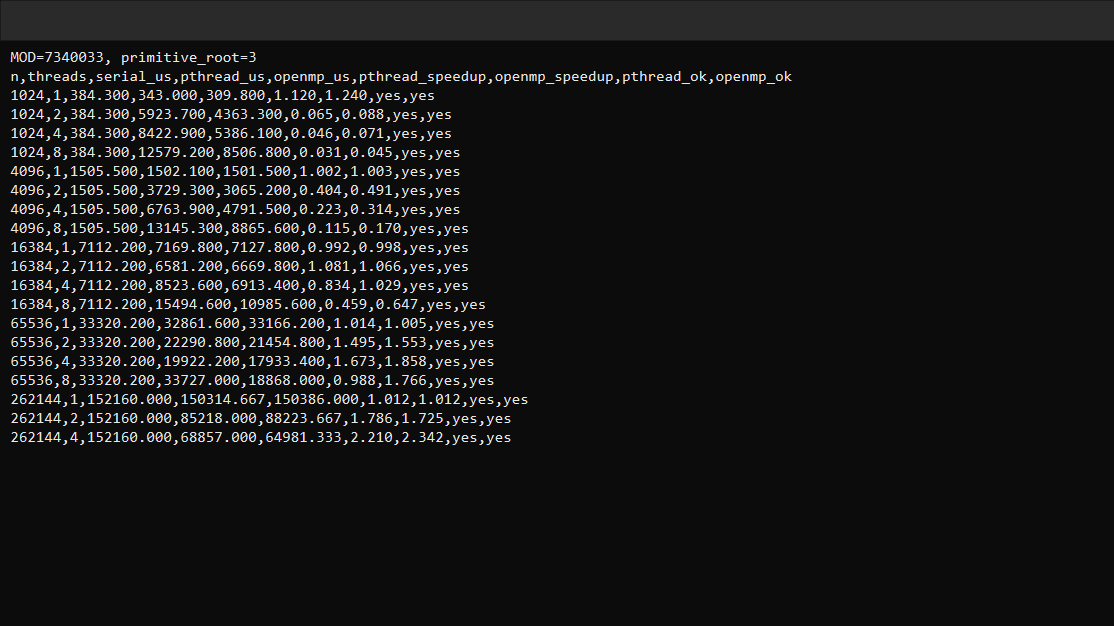
\includegraphics[width=0.96\textwidth]{assets/local_result_1.png}
\caption{本地平台运行结果截图（一）}
\label{fig:local-result-1}
\end{figure}

\begin{figure}[H]
\centering
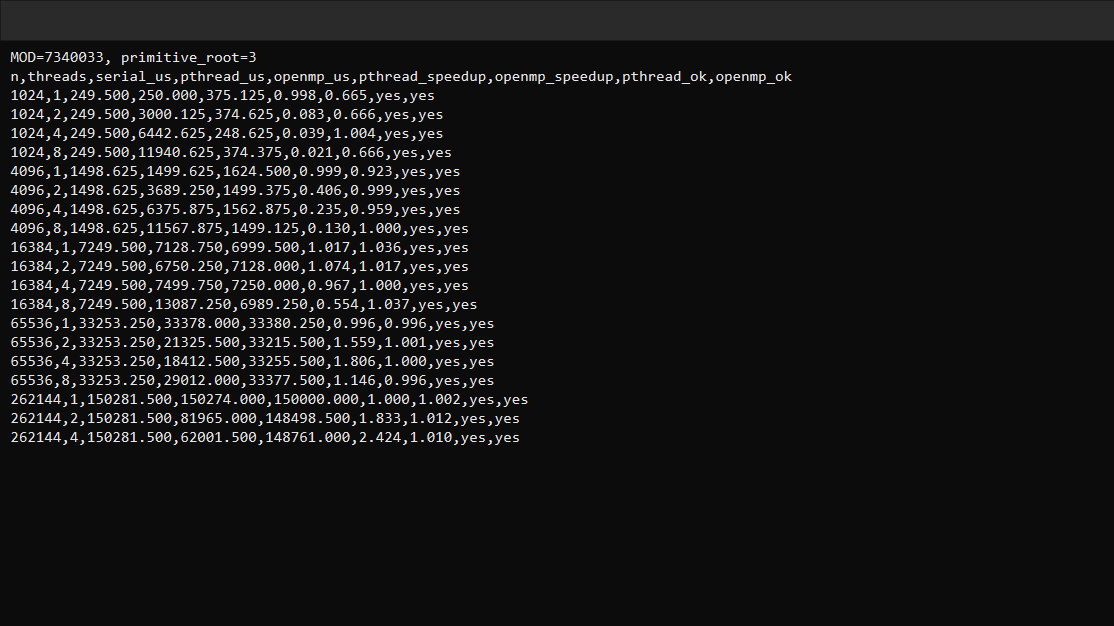
\includegraphics[width=0.96\textwidth]{assets/local_result_2.png}
\caption{本地平台运行结果截图（二）}
\label{fig:local-result-2}
\end{figure}

\begin{figure}[H]
\centering
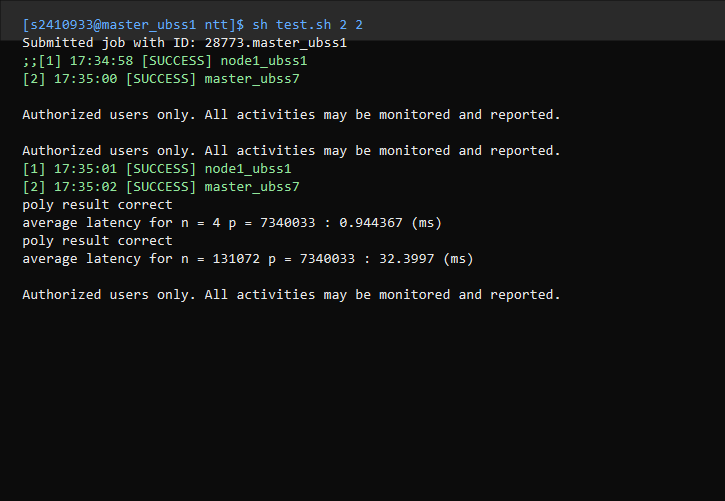
\includegraphics[width=0.78\textwidth]{assets/ssh_result_lab3.png}
\caption{SSH 平台运行结果截图}
\label{fig:ssh-result-lab3}
\end{figure}

\begin{figure}[H]
\centering
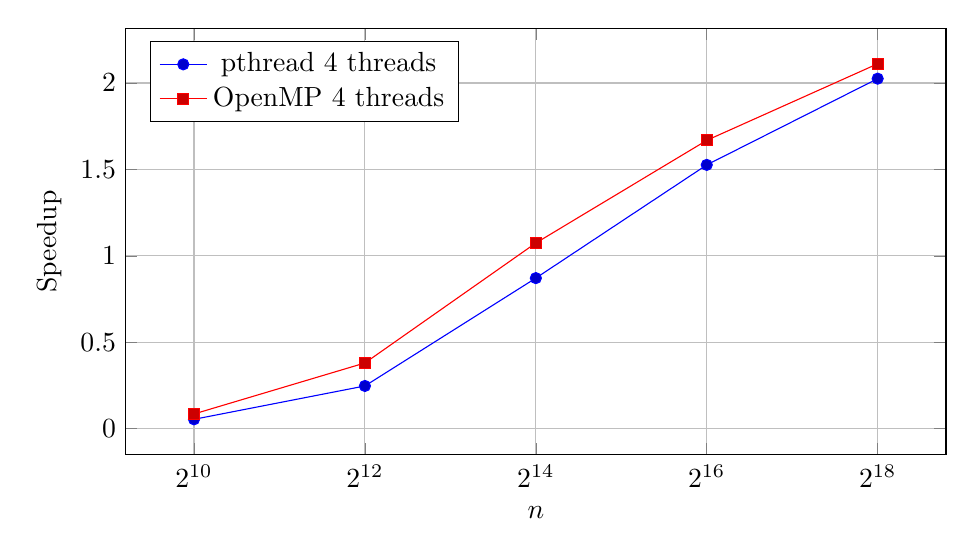
\begin{tikzpicture}
\begin{axis}[
    xlabel={$n$},
    ylabel={Speedup},
    grid=both,
    width=12cm,
    height=7cm,
    legend pos=north west,
    xtick={1024,4096,16384,65536,262144},
    xmode=log,
    log basis x={2}
]
\addplot coordinates {
(1024,0.054)
(4096,0.247)
(16384,0.871)
(65536,1.526)
(262144,2.025)
};
\addlegendentry{pthread 4 threads}
\addplot coordinates {
(1024,0.085)
(4096,0.380)
(16384,1.074)
(65536,1.668)
(262144,2.111)
};
\addlegendentry{OpenMP 4 threads}
\end{axis}
\end{tikzpicture}
\caption{4 线程下 pthread 与 OpenMP 加速比}
\end{figure}

\begin{figure}[H]
\centering
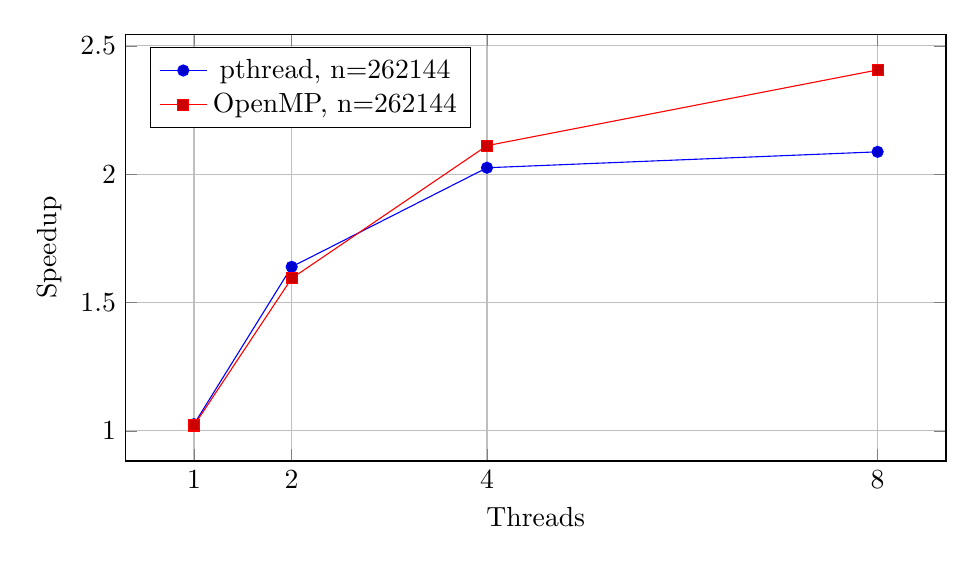
\begin{tikzpicture}
\begin{axis}[
    xlabel={Threads},
    ylabel={Speedup},
    grid=both,
    width=12cm,
    height=7cm,
    legend pos=north west,
    xtick={1,2,4,8}
]
\addplot coordinates {
(1,1.026)
(2,1.639)
(4,2.025)
(8,2.087)
};
\addlegendentry{pthread, n=262144}
\addplot coordinates {
(1,1.021)
(2,1.594)
(4,2.111)
(8,2.406)
};
\addlegendentry{OpenMP, n=262144}
\end{axis}
\end{tikzpicture}
\caption{$n=262144$ 时不同线程数加速比}
\end{figure}

\section{性能分析}

\subsection{小规模性能下降}

在 $n=1024$ 和 $n=4096$ 时，多线程版本明显慢于串行版本。仔细想是合理的：这两个规模下 NTT 每一层的计算量并不大，而 pthread 版本在每一层需要两次 barrier 同步，OpenMP 版本也需要在每一层完成 \texttt{single} 与 \texttt{for} 的同步。线程同步、运行时调度和 cache 抖动的开销超过了并行计算带来的收益。

这也说明，并行化并不是无条件有效的。当任务粒度太小时，额外开销会主导总时间，串行执行反而更合适。

\subsection{大规模加速效果}

当 $n$ 增大到 $65536$ 和 $262144$ 后，每一层包含的 butterfly 数量明显增加，线程同步开销被更多计算摊薄。$n=262144$ 时，pthread 8 线程加速比达到 2.087，OpenMP 8 线程达到 2.406，这说明同层 butterfly 并行确实能够利用多核资源。

不过 pthread 8 线程在 $n=65536$ 和 $n=262144$ 下没有继续显著提升。可能原因包括：
\begin{enumerate}
  \item 每一层都需要同步，线程数增加后等待最慢线程的代价提高；
  \item 多线程同时读写同一数组的不同位置，内存带宽和 cache 一致性开销增加；
  \item NTT 的后几层单个 block 较大，访问跨度变化会影响 cache 局部性；
  \item pthread 版本每次 NTT 变换显式创建线程，虽然避免了每层创建线程，但仍有一定线程管理成本。
\end{enumerate}

\subsection{pthread 与 OpenMP 对比}

这次写完两版以后，我对 pthread 和 OpenMP 的差异感受更明显。pthread 的优点是控制更直接，可以明确安排 barrier 和 task 分配策略；缺点是代码量更大，线程生命周期、同步和错误处理都需要手工管理。OpenMP 的代码明显更简洁，运行时线程池和调度机制也比较成熟，因此在本实验大规模数据下表现略优。

从实验结果看，OpenMP 在 $n=65536$、$n=262144$ 时整体优于 pthread，尤其是 8 线程下更明显。一个重要原因可能是 OpenMP 版本按照实验文档建议，把并行区域放在 NTT 主循环外部，减少了反复 fork-join 的开销；而当前 pthread 版本是在每次 NTT 变换中重新创建工作线程。

\section{实验中遇到的问题}

\subsection{旋转因子递推与并行冲突}

串行版本中每个 block 内的旋转因子通过变量 $w$ 递推。如果直接并行化最内层循环，不同线程会破坏 $w$ 的递推关系。为了解决这个问题，程序在每一层预先生成旋转因子表 \texttt{roots[k]}，每个 task 直接读取对应的旋转因子，从而让 butterfly 之间真正变成独立任务。

\subsection{同步粒度选择}

如果每个 block 或每个 butterfly 都使用锁，会产生非常高的同步开销。根据 NTT 的依赖关系，其实只需要在层与层之间同步即可。因此最终采用每层两个 barrier：一个保证旋转因子表生成完成，另一个保证本层 butterfly 全部完成。

\section{结论}

本次实验完成了 NTT 卷积的串行、pthread 和 OpenMP 三种实现，并在多组规模和线程数下进行了正确性与性能测试。根据实验结果，可以得到以下结论：

\begin{enumerate}
  \item NTT 同一层的 butterfly 操作互不冲突，适合进行线程级并行；
  \item 多线程版本在所有测试中都与串行结果完全一致；
  \item 小规模下线程同步和调度开销会超过计算收益，导致多线程变慢；
  \item 大规模下 pthread 和 OpenMP 均取得明显加速，$n=262144$ 时 OpenMP 8 线程加速比达到 2.406；
  \item OpenMP 代码更简洁，在本实验环境中大规模性能也略优；pthread 版本提供了更细粒度的控制，但还可以通过跨 NTT 调用复用线程池继续优化。
\end{enumerate}

总体来看，NTT 的多线程优化重点不只是“把循环拆给多个线程”，还需要在并行粒度、同步开销和内存访问之间做权衡。只有当单层 butterfly 数量足够大时，多线程才能稳定带来性能收益。

\end{document}
